\documentclass[10pt, portrait]{article}
\usepackage[scaled=0.92]{helvet}
\usepackage{calc}
\usepackage{multicol}
\usepackage{ifthen}
\usepackage[a4paper,margin=5mm,portrait]{geometry}
\usepackage{amsmath,amsthm,amsfonts,amssymb}
\usepackage{color,graphicx,overpic}
\usepackage{hyperref}
\usepackage{newtxtext} 
\usepackage{enumitem}
\usepackage{amssymb}
\usepackage[table]{xcolor}
\usepackage{vwcol}
\usepackage{tikz}
\usetikzlibrary{arrows.meta}
\usetikzlibrary{calc}
\usepackage{mathtools}
\usepackage{nicematrix}
\usepackage[T1]{fontenc} %%% <--- NOTE THIS
% for relations
\usepackage{cancel}
\usepackage{ mathrsfs }
\usepackage{listings}
\usepackage{background}
\setlist{nosep}

\backgroundsetup{
scale=1,
color=black,
opacity=0.3,
angle=0,
contents={%
  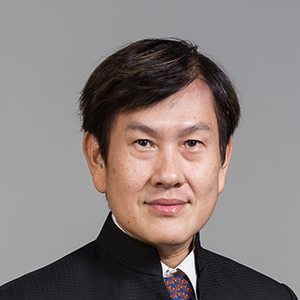
\includegraphics[width=\paperwidth,height=\paperheight]{tantc.jpg}
  }%
}

\pdfinfo{
  /Title (CS2100.pdf)
  /Creator (TeX)
  /Producer (pdfTeX 1.40.0)
  /Author (Seamus)
  /Subject (Example)
  /Keywords (pdflatex, latex,pdftex,tex)}

\lstset{language=Java,keywordstyle={\bfseries \color{black}}}

% Turn off header and footer
\pagestyle{empty}

\newenvironment{tightcenter}{%
  \setlength\topsep{0pt}
  \setlength\parskip{0pt}
  \begin{center}
}{%
  \end{center}
}

% redefine section commands to use less space
\makeatletter
\renewcommand{\section}{\@startsection{section}{1}{0mm}%
                                {-1ex plus -.5ex minus -.2ex}%
                                {0.5ex plus .2ex}%x
                                {\normalfont\large\bfseries}}
\renewcommand{\section}{\@startsection{section}{2}{0mm}%
                                {-1explus -.5ex minus -.2ex}%
                                {0.5ex plus .2ex}%
                                {\normalfont\normalsize\bfseries}}
\renewcommand{\subsection}{\@startsection{subsection}{3}{0mm}%
                                {-1ex plus -.5ex minus -.2ex}%
                                {1ex plus .2ex}%
                                {\normalfont\small\bfseries}}%
\renewcommand{\familydefault}{\sfdefault}
\renewcommand\rmdefault{\sfdefault}
% makes nested numbering (e.g. 1.1.1, 1.1.2, etc)
\renewcommand{\labelenumii}{\theenumii}
\renewcommand{\theenumii}{\theenumi.\arabic{enumii}.}
\renewcommand\labelitemii{•}
%  for logical not operator
\renewcommand{\lnot}{\mathord{\sim}}
\renewcommand{\bf}[1]{\textbf{#1}}
\newcommand{\abs}[1]{\vert #1 \vert}
\newcommand{\Mod}[1]{\ \mathrm{mod}\ #1}

\makeatother
\definecolor{myblue}{cmyk}{1,.72,0,.38}
\everymath\expandafter{\the\everymath \color{myblue}}
% Define BibTeX command
\def\BibTeX{{\rm B\kern-.05em{\sc i\kern-.025em b}\kern-.08em
    T\kern-.1667em\lower.7ex\hbox{E}\kern-.125emX}}
\let\iff\leftrightarrow
\let\Iff\Leftrightarrow
\let\then\rightarrow
\let\Then\Rightarrow

% Don't print section numbers
\setcounter{secnumdepth}{0}

\setlength{\parindent}{0pt}
\setlength{\parskip}{0pt plus 0.5ex}
%% this changes all items (enumerate and itemize)
\setlength{\leftmargini}{0.5cm}
\setlength{\leftmarginii}{0.5cm}
\setlist[itemize,1]{leftmargin=2mm,labelindent=1mm,labelsep=1mm}
\setlist[itemize,2]{leftmargin=4mm,labelindent=1mm,labelsep=1mm}

%My Environments
\newtheorem{example}[section]{Example}
% -----------------------------------------------------------------------

\begin{document}
\raggedright
\footnotesize
\begin{multicols*}{2}


% multicol parameters
% These lengths are set only within the two main columns
\setlength{\columnseprule}{0.25pt}
\setlength{\premulticols}{1pt}
\setlength{\postmulticols}{1pt}
\setlength{\multicolsep}{1pt}
\setlength{\columnsep}{2pt}

\begin{center}
    \fbox{%
        \parbox{0.8\linewidth}{\centering \textcolor{black}{
            {\Large\textbf{CS2100}}
            \\ \normalsize{AY24/25 Sem 2}}
            \\ {\footnotesize \textcolor{myblue}{by ngmh}} 
        }%
    }
\end{center}

\section{1. Introduction}
\begin{itemize}
    \item Programming Language: A formal language that specifies a set of instructions for a computer to implement specific algorithms to solve problems
    \item High-Level: Level of abstraction closer to problem domain, provides productivity and portability
    \item Assembly Language: Textual and symbolic representation of instructions
    \item Machine Code: Binary bits of instructions and data
    \item von Neumann Architecture: Computer consisting of Input Device, Central Processing Unit (Control Unit, ALU), Memory Unit, Output Device
\end{itemize}

\section{2. C Programming}
\begin{itemize}
    \item Edit, Compile, Execute
    \item C Program Format
    \begin{verbatim}
    preprocessor directives

    main function header {
        declaration of variables
        executable statements
    }
    \end{verbatim}
    \item Uninitialised variables do not necessarily contain zero
    \item Variables consist of address, name, data type, and value
    \item Data types: int (4 bytes), float (4 bytes), double (8 bytes), char (1 byte)
    \item C is strongly typed
    \item Preprocessor Directives: Inclusion of header files, Macro Expansions
    \item Input / Output : scanf, printf, remember address for scanf
    \item Format Specifier: c (char), d (int), f (float), lf (double), e (float or double)
    \item $\%n.mf$ means width $n$ including $m$ decimal places
    \item \%\% for literal \%
    \item Boolean expressions can be short-circuited
\end{itemize}

\section{3. Number Systems}
\begin{itemize}
    \item Data is stored as bits
    \item Byte: 8 bits, Nibble: 4 bits, Word: Multiple of Bytes
    \item $N$ bits can represent $2^N$ values, $M$ values require $\lceil log_2M \rceil$ bits
    \item Weighted-Positional Number System: Left is increasing powers, Right is decreasing powers
    \item Number Systems: Decimal (Base 10), Binary (Base 2 / 0b), Octal (Base 8 / 0), Hexadecimal (Base 16 / 0x)
    \item Base-R to Decimal: Multiplication by weights and summation
    \item Decimal to Binary Conversion: Repeated Multiplication / Division by 2 (Works for other bases as well)
    \item Repeated Divison by 2:
    \begin{verbatim}
    43 (10) = 101011 (2)
    21 r 1 LSB
    10 r 1
    5 r 0
    2 r 1
    1 r 0
    0 r 1 MSB
    \end{verbatim}
    \item Repeated Multiplication by 2:
    \begin{verbatim}
    0.3125 (10) = 0.0101 (2)
    0.625 c 0 MSB
    1.250 c 1
    0.500 c 0
    1.000 c 1 LSB
    \end{verbatim}
    \item For conversion with other bases, use Base-10 as intermediary
    \item Between bases of multiples of 2, simplify partition or split characters
    \item ASCII: 7 bits + 1 parity bit (used as checksum)
    \item Odd Scheme: Parity after adding parity bit must be odd
    \item Unsigned Numbers: Only non-negative values (as opposed to signed)
    \item Overflow: Result of addition or subtraction goes out of range, can be detected by checking if sign of result matches
\end{itemize}

\subsection{Sign-and-Magnitude}
\begin{itemize}
    \item 1 sign bit (MSB), other bits for magnitude
    \item Sign: 0 is positive, 1 is negative
    \item Range: $-(2^{n-1}-1)$ to $2^{n-1}-1$
    \item Has redundant zero
    \item Negation: Just invert sign bit
\end{itemize}

\subsection{1s Complement}
\begin{itemize}
    \item $-x=2^n-x-1$
    \item Sign: See MSB
    \item Negation: Invert all bits
    \item Range: $-(2^{n-1}-1)$ to $2^{n-1}-1$
    \item Has redundant zero
    \item Addition: Perform binary addition, adding 1 to the result if there is carry out due to redundant zero
    \item Subtraction: Perform addition with negation of the second term
\end{itemize}

\subsection{2s Complement}
\begin{itemize}
    \item $-x=2^n-x$
    \item Sign: See MSB
    \item Negation: Invert all bits, then add 1
    \item Range: $-2^{n-1}$ to $2^{n-1}-1$
    \item No redundant zero
    \item Addition: Perform binary addition, ignoring carry out
    \item Subtraction: Perform addition with negation of second term
\end{itemize}

\subsection{Excess Representation}
\begin{itemize}
    \item Allows range of values to be distributed evenly between positive and negative values by a simple translation
    \item Value $v$ is represented as $v+n$ in Excess $n$
    \item Range: $-n$ to $n-1$
    \item For even distributio of $k$-bit numbers we should use Excess-$2^{k-1}$ or Excess-$2^{k-1}-1$
\end{itemize}

\subsection{Radix Complement}
\begin{itemize}
    \item For number of digits $n$ and radix $b$
    \item $(b-1)$s Complement: $-x=b^n-x-1$
    \item $(b)$s Complement: $-x=b^n-x$
\end{itemize}

\subsection{Fraction Extension}
\begin{itemize}
    \item For $n$ bits and $f$ fractional bits
    \item $1$s Complement: $-x=2^n-x-2^{-f}$, invert all bits
    \item $2$s Complement: $-x=2^n-x$, invert all bits, add $2^{-f}$ (the smallest bit)
    \item Resolution is the smallest bit value
    \item Might have to round off if non-exact
\end{itemize}

\subsection{Real Numbers}
\begin{itemize}
    \item Fixed Point Representation: Number of bits allocated for whole number part and fractional part
    \item IEEE754 Floating Point Representation:
    \begin{itemize}
        \item Sign, Exponent, Mantissa (Fraction)
        \item Single Precision: 1-bit sign, 8-bit exponent in excess-127, 23-bit mantissa
        \item Double Precision: 1-bit sign, 11-bit exponent in excess-1023, 52-bit mantissa
        \item Sign: 0 for positive, 1 for negative
        \item Mantissa is normalised, with implicit leading bit 1 (e.g. $110.1 = 1.101 \times 2^2$)
        \item Exponent is stored in excess-127 (e.g. $2+127=129$
        \item Merge components together and express in hexadecimal
    \end{itemize}
\end{itemize}

\section{4. Pointers and Functions}
\subsection{Pointers}
\begin{itemize}
    \item The address of a variable can be found with \&, and has format specifier p
    \item Pointers store these addresses, along with the data type they are pointing to
    \item They are defined using *
    \item Dereference pointers using *
    \item Incrementing a pointer moves its value by the data type size
\end{itemize}

\subsection{Functions}
\begin{itemize}
    \item User-Defined Functions: Require prototype before main, and definition after main
    \item Function Prototype: Return type, method name, types of parameters (name optional)
    \item Use void in prototype of function with no parameters, empty means unspecified
    \item C parameters are pass by value
    \item Scope Rule: Local variables are only accessible within function they are declared
    \item Can use static to make values persistent across calls
    \item Function can take in pointers instead to achieve pass by reference
\end{itemize}

\section{5. Arrays, Strings and Structures}
\subsection{Arrays}
\begin{itemize}
    \item Homogeneous collection of data
    \item Declared by element type, array name, and size
    \item Elements are 0-indexed
    \item Arrays can be initialised only at declaration
    \item Array name is a fixed constant pointer and cannot be altered
    \item Address and value of array variable are always the same
    \item In function parameters, need to specify [] to show it is an array or simplify take in a pointer instead
    \item Functions involving arrays need size parameters as arrays decay into pointers when passed as parameters by array name
\end{itemize}

\subsection{Strings}
\begin{itemize}
    \item A string is an array of characters terminated by the null character \textbackslash 0
    \item Can be initialised directly with a string
    \item Input: fgets(str, size, stdin) or scanf("\%s", str)
    \item Output: puts(str) or printf("\%s", str)
    \item fgets() also reads in the newline character, so we might have to replace it
    \item puts() automatically adds a newline
    \item Some string functions include strlen(), strcmp(), strncmp(), strcpy(), strncpy()
    \item A non-null terminated string might cause illegal access of memory
\end{itemize}

\subsection{Structures}
\begin{itemize}
    \item Allow grouping of heterogeneous members
    \begin{verbatim}
    typedef struct {
        int acctNum;
        float balance;
    } account_t;
    \end{verbatim}
    \item Type declaration, not a variable
    \item Initialisation is similar to arrays
    \item Members are accessed using .
    \item Assignments are okay, unlike arrays
    \item Structs can also be passed into functions by value and returned from functions
    \item Entire contents even arrays are copied when they are passed by value
    \item Can use arrow operator $->$ instead of $(*).$
\end{itemize}

\section{7. MIPS Introduction}
\subsection{Overview}
\begin{itemize}
    \item Instruction Set Architecture: Abstraction on the interface between hardware and the low-level software
    \item Machine Code: Instructions in binary / hexadecimal, Hard and tedious to code
    \item Assembly: Human readable, Easier to write than machine code, symbolic version, may also provide pseudo-instructions as syntactic sugar
    \item A computer has processor and memory, with a bus acting as the bridge between them
    \item Code and data reside in memory, to be transferred into the processor during execution
    \item To avoid having to frequently access memory, the processor has temporary storage for values known as registers
    \item Need memory instructions to move data between registers as well as to and from memory
    \item Need arithmetic instructions as well, some of which involve constants
    \item Need instructions to manage control flow
\end{itemize}

\subsection{Registers}
\begin{itemize}
    \item Processor has fast memory in the form of registers
    \item Typical architecture has 16 to 32 registers, which the compiler associates with variables
    \item Registers have no data type
    \item MIPS has 32 registers (refer to Green Card)
\end{itemize}

\subsection{Language and Basic Operations}
\begin{itemize}
    \item Each instruction executes a simple command
    \item Each line has at most 1 instruction
    \item Use \# for comments
    \item Operation followed by destination then sources
    \item e.g. add \$rd, \$rs, \$rt
    \item Immediate operation: Has an immediate instead of second argument which uses 16 bit 2s complement
    \item Immediate is sign extended, meaning the MSB is duplicated all the way across the upper half, which is actually value preserving
    \item subi does not exist, use addi with negative constant
    \item Register \$zero is guaranteed to have a zero value
    \item Bit shifting is limited to 5 bits as registers are only 32 bits
    \item not does not exist, use nor \$t0, \$t0, \$zero instead
    \item To load large constants, we need to use lui to set the upper bits, and ori to set the lower bits
    \item Basic Operations:
\end{itemize}
\begin{center}
    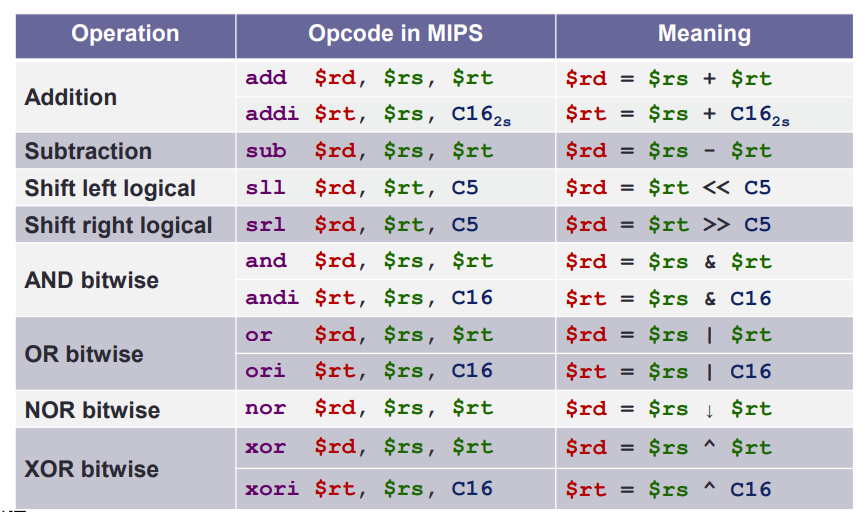
\includegraphics[width=0.7\linewidth]{mips basic.png}
\end{center}

\section{8. More Instructions}
\subsection{Memory Instructions}
\begin{itemize}
    \item The main memory can be viewed as a large single dimension array
    \item Each location of the memory has an address
    \item We can use addresses to access a single byte / word
    \item A word usually has a size which is a power of 2, and usually coincides with register size
    \item Word Alignment: Words that are aligned in memory begin at a byte address which is a multiple of word size
    \item lw / sw \$t0, 4(\$s0)
    \item Address is offset from a base address, and must be word aligned
\end{itemize}

\subsection{Control Flow}
\begin{itemize}
    \item Conditional: Branching
    \item Unconditional: Jumping
    \item beq \$r1, \$r2, label
    \item Jump to statement with label if values in registers are equal
    \item Labels represent instruction addresses and are not instructions
    \item To produce shorter code, invert the condition in C code to favor early exit
    \item Use combination of branching and jumps to make a for loop
    \begin{verbatim}
        add $s0, $zero, $zero
        addi $s1, $zero, 10
    Loop: beq $s0, $s1, Exit
        addi $s2, $s2, 5
        addi $s0, $s0, 1
        j Loop
    Exit:
    \end{verbatim}
    \item Use slt (set less than) to simulate comparisons
\end{itemize}

\section{9. MIPS Instruction Formats and Encoding}
\begin{itemize}
    \item Every MIPS instruction is 32 bits long
    \item Register Format: op \$r1, \$r2, \$r3
    \item Immediate Format: op \$r1, \$r2, Immd
    \item Jump Format: op Immd
    \item Refer to Green Card for more information
\end{itemize}

\subsection{R-Format}
\begin{itemize}
    \item opcode: Specifies instruction, 0 for all R-format instructions
    \item funct: Combines with opcode to specify instruction
    \item rs: Specifies source register
    \item rt: Specifies target register
    \item rd: Specifies destination register
    \item shamt: Bit shift amount
\end{itemize}

\subsection{I-Format}
\begin{itemize}
    \item Bigger field for intermediate values
    \item rt is destination register instead as there is no rd
    \item immediate: 16 bits signed integer in 2s complement
\end{itemize}

\subsection{Addressing}
\begin{itemize}
    \item Since instructions are stored in memory, they also have addresses which are word aligned
    \item Program Counter: Special register that keeps address of instruction being executed in processor
    \item Conditional instructions are I-format and use immediate for PC-relative addressing
    \item Immediate is specified as target address relative to PC, as a number of words
    \item If branch is not taken, $PC = PC + 4$
    \item If branch is taken, $PC = (PC+4)+(Immd \times 4)$
    \item Start counting from next line of code
\end{itemize}

\subsubsection{Addressing Modes}
\begin{itemize}
    \item Register Addressing: Operand are all registers
    \item Immediate Addressing: Operand is a constant within instruction itself
    \item Base Addressing / Displacement Addressing: One of the register operands is a memory location while another immediate value corresponds to the offset from the given memory location
    \item PC-Relative Addressing: Base address is given by PC register
    \item Pseudo-Direct Addressing: Use only upper 4-bits of PC register, with rest of address being obtained from instruction, with last 2 bits 00 due to word alignment
\end{itemize}

\subsection{J-Format}
\begin{itemize}
    \item Allows jumps to further locations through psuedo-direct addressing
    \item Target address field is only 26 bits however
    \item But since instructions are word aligned, we can assume the last 2 bits to be 00
    \item The remaining 4 bits are taken from the MSB of PC+4
    \item Jump boundary is now 256MB
\end{itemize}

\section{10. Instruction Set Architecture}
\begin{itemize}
    \item Complex Instruction Set Computer (CISC): Single instruction performs complex operation, smaller program size, but complex implementation which does not leave room for hardware optimisation (e.g. x86-32)
    \item Reduced Instruction Set Computer (RISC): Simple instruction set, easier to optimise hardware, but burden is on software to implement high-level language statements (e.g. MIPS, ARM)
\end{itemize}

\subsection{Data Storage}
\begin{itemize}
    \item Storage Architecture: How are operands and computation results stored
    \item Stack Architecture: Operands are implicitly on top of stack
    \item Accumulator: One operand is implicitly in the accumulator (a special register)
    \item General-Purpose Register Architecture: Only explicit operands (Register-Memory, Register-Register / Load-Store)
    \item Memory-Memory Architecture: All operands in memory
    \item The most common is general-purpose register, with RISC using Register-Register design and CISC using a mix of both
\end{itemize}
\begin{center}
    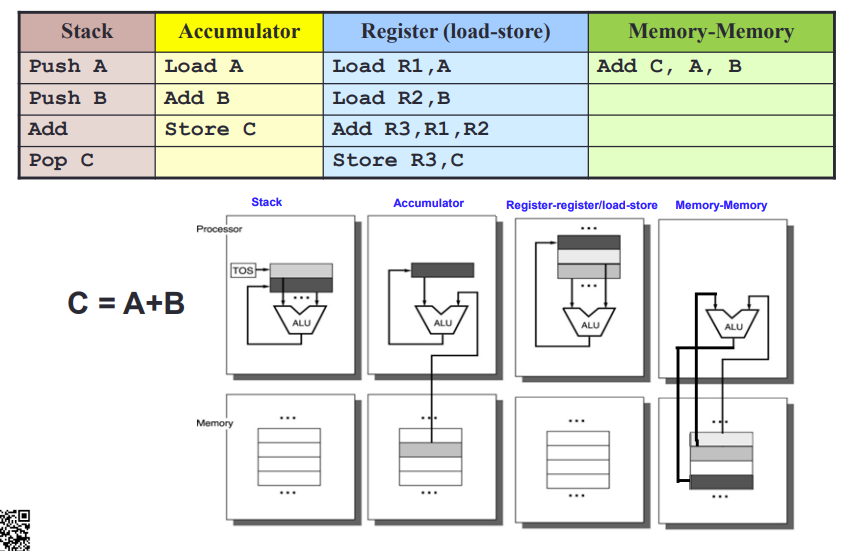
\includegraphics[width=\linewidth]{architecture.png}
\end{center}

\subsection{Memory Addressing Mode}
\begin{itemize}
    \item Give $k$-bit addresses, the address space has size $2^k$ with each memory transfer consisting of one word of $n$ bits
    \item Endianness: Relative ordering of bytes in a multiple-byte word store in memory
    \item Big-Endian: MSB stored in lowest address (e.g. MIPS)
    \item Little-Endian: LSB stored in lowest address
    \item Addressing Modes in MIPS: Register, IMmmediate, Displacement
\end{itemize}

\subsection{Operations}
\begin{itemize}
    \item Standard Operation Types:
    \begin{itemize}
        \item Data Movement
        \item Arithmetic, Shift, Logical
        \item Control Flow, Subroutine Linkage
        \item Interrupt
        \item Synchronisation, String, Graphics
    \end{itemize}
    \item Frequently used instructions should be made the fastest
\end{itemize}

\subsection{Instruction Formats}
\begin{itemize}
    \item Instruction Length
    \begin{itemize}
        \item Variable-length: Require multi-step fetch and decode, more flexibility but more complex
        \item Fixed-length: Used in most RISCs, allow for easy fetch and decode, simplifies pipelining and parallelism, but instruction bits are scarce
        \item Hybrid: Mix of both
    \end{itemize}
    \item Instruction Fields
    \begin{itemize}
        \item Type and Size of operands
        \item Consists of opcode and operands
        \item Typical type and sizes include characters (1 byte), word, floating points with single and double precision (1 / 2 words)
    \end{itemize}
\end{itemize}

\subsection{Encoding the Instruction Set}
\begin{itemize}
    \item Instruction Encoding
    \begin{itemize}
        \item How are instructions represented in binary format
        \item Variable v/s Fixed v/s Hybrid
        \item Number of registers, adressing modes, number of operands
    \end{itemize}
    \item Encoding Fixed Length Instructions
    \begin{itemize}
        \item Expanding Opcode Scheme: Opcode has variable lengths for different instructions
        \item Example: 16 bit instructions, 2 types of instructions
        \item Type A: 2 operands, each 5 bits
        \item Type B: 1 operand, 5 bits
        \item Maximum Number: Minimise Type A, $1 + (2^6-1) \times 2^5=2017$
        \item Minimum Number: Maximise Type A, $(2^6-1) + 1 \times 2^5=95$
    \end{itemize}
\end{itemize}

\section{11. MIPS Datapath}
\begin{itemize}
    \item Processor has Datapath: Collection of components that process data and performs arithmetic, logical, and memory operations
    \item It also has Control: Tells the datapath, memory, and I/O devices what to do according to program instructions
    \item Basic Instruction Execution Cycle
    \begin{itemize}
        \item Fetch: Get instruction from memory, address is in PC
        \item Decode: Find out the operation required
        \item Operand Fetch: Get operands needed for operation
        \item Execute: Perform the required operation
        \item Result Write (Store): Store the result of the operation
    \end{itemize}
    \item MIPS Instruction Execution
    \begin{itemize}
        \item Decode and Operand Fetch are merged as decoding is simple
        \item Execute is split into ALU (Calculation) and Memory Access
    \end{itemize}
\end{itemize}

\subsection{Building a MIPS Processor}
\subsubsection{Fetch Stage}
\begin{itemize}
    \item Use PC to fetch instruction from memory
    \item Increment PC by 4 to get address of next instruction
    \item Output the instruction to be executed to the decode stage
    \item Instruction Memory:
    \begin{itemize}
        \item Storage element for instructions, functions like a big array
        \item Is a sequential circuit
        \item Has internal state that stores information
        \item Clock signal is assumed and not shown
        \item Supplies instruction when given an address
    \end{itemize}
    \item Adder: Combinational logic to implement addition of two numbers, has no state
    \item Clocking: Read and update PC at the same time by performing each action at different parts of the clock cycle, update is only performed at rising edge
\end{itemize}
\begin{center}
    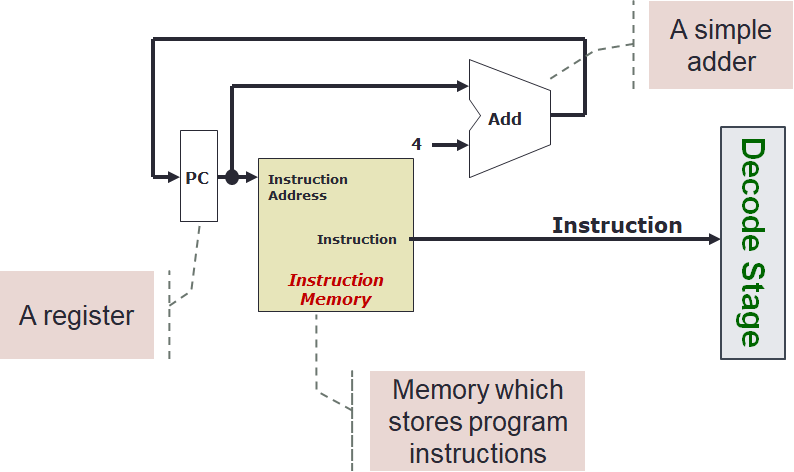
\includegraphics[width=0.7\linewidth]{fetch.png}
\end{center}

\subsubsection{Decode Stage}
\begin{itemize}
    \item Gather data from instruction fields: opcode and data from necessary registers
    \item Input instruction is taken from fetch stage
    \item Output operation and necessary operands to ALU stage
    \item Register File: \begin{itemize}
        \item Collection of 32 registers
        \item Each register is 32 bit, and at most two are read and one written
        \item RegWrite: Control signal to indicate writing of register (1 is write, 0 is no write)
    \end{itemize}
    \item Problems
    \begin{itemize}
        \item Not all instructions have destination in the same place
        \item Multiplexer and RegDst control signal is used to determine where to read from
        \item Read Data 2 might be an immediate value instead of a register input
        \item Multiplexer is used to choose the correct operand, with sign extension applied to 16-bit immediate to make it 32-bit
    \end{itemize}
    \item Multiplexer:
    \begin{itemize}
        \item Selects one input from multiple input lines
        \item Input: $n$ lines of same width
        \item Control: $m$ bits where $n=2^m$
        \item Output: Select the $i^{th}$ input line based on control
    \end{itemize}
\end{itemize}
\begin{center}
    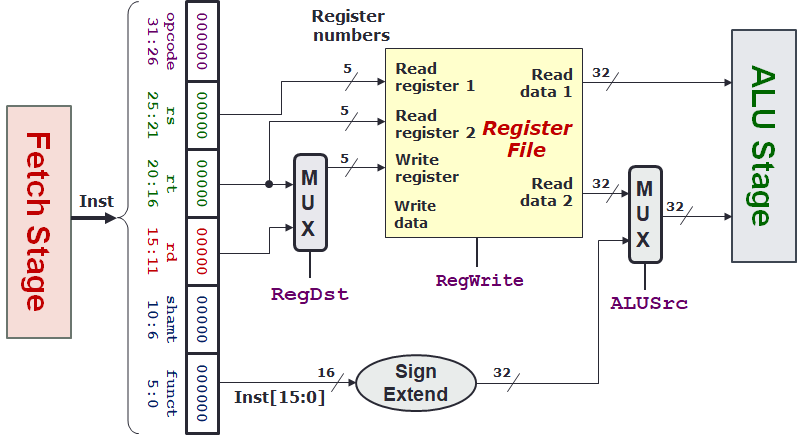
\includegraphics[width=0.7\linewidth]{decode.png}
\end{center}

\subsubsection{ALU Stage}
\begin{itemize}
    \item Arithmetic Logic Unit
    \item a.k.a Execution Stage
    \item Perform real work for most instructions
    \item Input operation and operands are from decode stage
    \item Output calculation result is given to memory stage
    \item ALU
    \begin{itemize}
        \item Combinational logic to implement arithmetic and logical operations
        \item Input: 2 32-bit numbers
        \item Control: 4-bit signal
        \item Output: Result of operation and 1-bit signal to indicate whether result is 0
    \end{itemize}
    \item Branch Instructions
    \begin{itemize}
        \item Branch Outcome: Determine using ALU for comparison and isZero? signal
        \item Branch Target Address: Introduce logic to calculate the address using PC from fetch stage and Offset from decode stage
    \end{itemize}
\end{itemize}
\begin{center}
    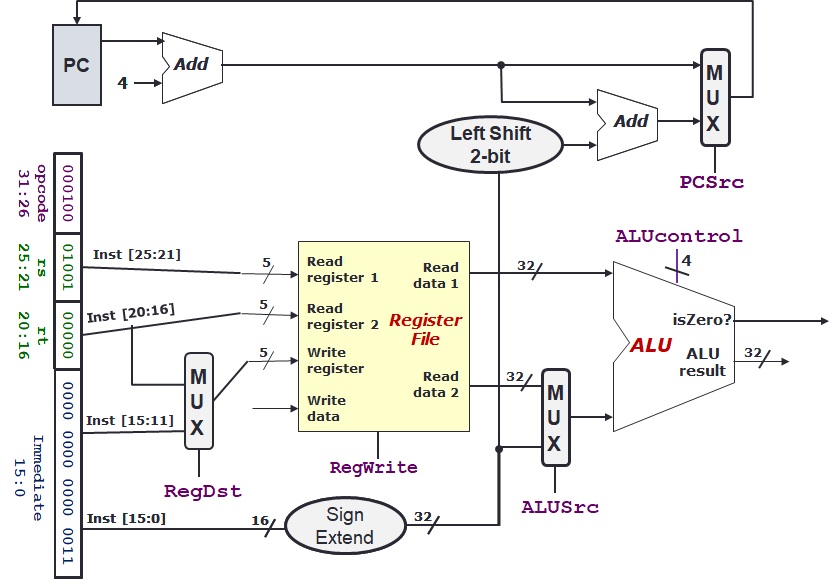
\includegraphics[width=0.7\linewidth]{alu.png}
\end{center}

\subsubsection{Memory Stage}
\begin{itemize}
    \item Only load and store operations are needed
    \item Use memory address calculated by ALU stage and read or write data memory
    \item All other instructions remain idle
    \item Input is computation result as memory address (if applicable) from ALU stage
    \item Output is result to be stored (if applicable) to register write stage
    \item Data Memory
    \begin{itemize}
        \item Storage element for data of program, functions like a big array
        \item Input: Memory Address, Data to be Written
        \item Control: Read and Write controls, only one at a time
        \item Output: Data read from memory for load instructions
    \end{itemize}
    \item Need Read Data 2 from decode stage as Write Data
    \item MemToReg: Control signal to indicate whether result came from memory or ALU unit, inverted
\end{itemize}
\begin{center}
    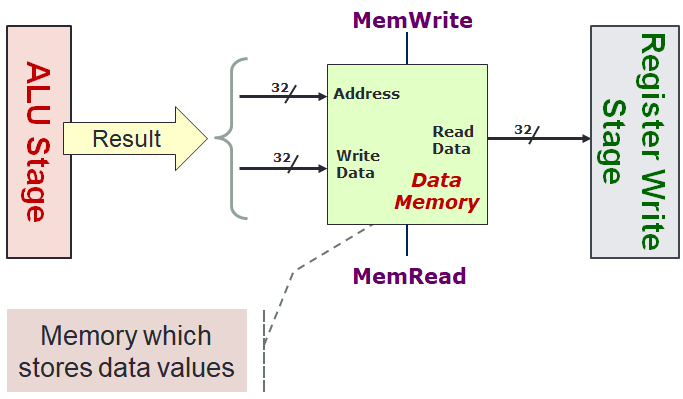
\includegraphics[width=0.7\linewidth]{memory.png}
\end{center}

\subsubsection{Register Write Stage}
\begin{itemize}
    \item Most instructions write the result of computation into a register
    \item Need destination register number and computation result
    \item Exceptions are stores, branches, and jumps
    \item Input is the computation result either from memory or ALU
    \item No additional elements, simply route correct result into register file, using Write Register number generated back in decode stage
\end{itemize}
\begin{center}
    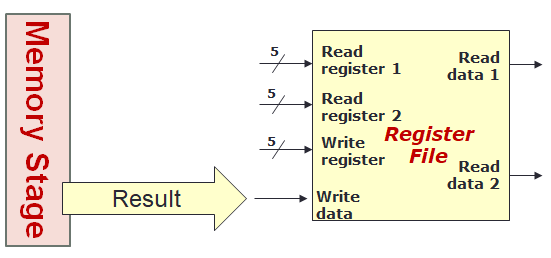
\includegraphics[width=0.7\linewidth]{write.png}
\end{center}

\subsection{Complete MIPS Datapath}
\begin{center}
    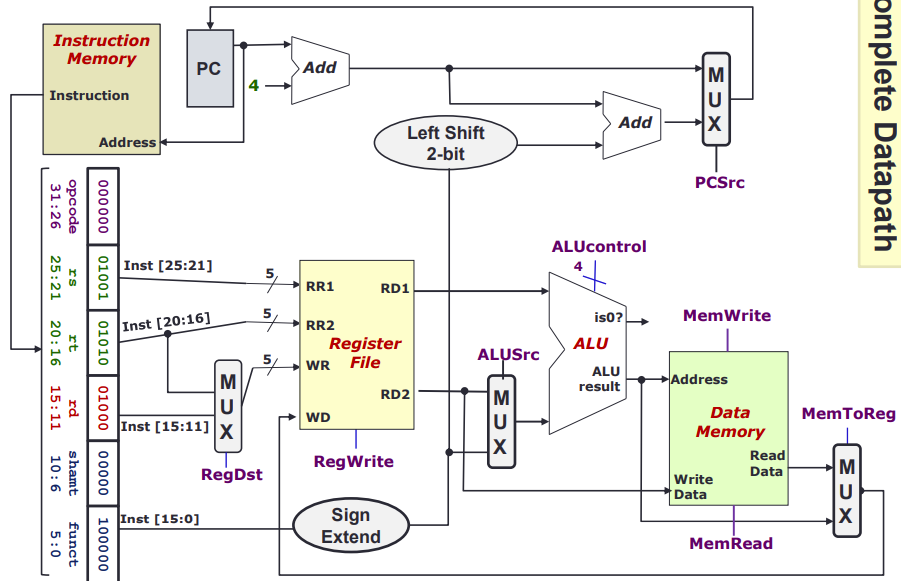
\includegraphics[width=\linewidth]{mips datapath.png}
\end{center}

\subsection{Compiling and Execution}
\begin{itemize}
    \item Compiler translate to high-level language to assembly language
    \item Assembler translates to machine code
    \item Processor executes the machine code
    \item Compiling to MIPS
    \begin{itemize}
        \item Compilation is structured, and each structure can be compiled independently
        \item Variable-to-Register Mapping
        \item Conditions can be inverted for shorter code
        \item Complex operations should be broken down with temporary registers
        \item Array access is lw while array update is sw
        \item Remember that word addresses differ by word size
    \end{itemize}
\end{itemize}

\section{12. MIPS Control}
\begin{itemize}
    \item Control signals are generated based on the instruction to be executed
    \item A control unit is needed to design a combinational circuit to generate signals based on opcode and possibly funct
    \item General Flow: Take note of instructions to be implemented, go through each signal to observe how it is generated, construct truth table, then design control unit using logic gates
    \item Logic Gates
\end{itemize}
\begin{center}
    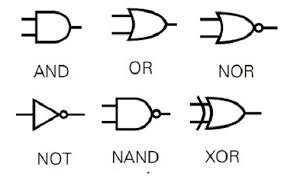
\includegraphics[width=0.5\linewidth]{gates.jpg}
\end{center}

\subsection{Control Signals}
\begin{itemize}
    \item RegDst:
    \begin{itemize}
        \item Selects destination register number
        \item False: False: Write Register = rt / Inst[20:16]
        \item True: Write Register = rd / Inst[15:11]
    \end{itemize}
    \item RegWrite:
    \begin{itemize}
        \item Enable writing of register
        \item False: No register write
        \item True: New value will be written
    \end{itemize}
    \item ALUSrc:
    \begin{itemize}
        \item Select second operand for ALU
        \item False: Operand2 = Register Read Data 2
        \item True: Operand2 = Immd / SignExt(Inst[15:0])
    \end{itemize}
    \item MemRead / MemWrite
    \begin{itemize}
        \item Enable reading / writing of data memory
        \item False: Not performing memory read access or memory write
        \item True: Read memory using Address / write register read data 2 to memory at address
    \end{itemize}
    \item MemToReg:
    \begin{itemize}
        \item Select result to be written back to register file
        \item True: Register Write Data = Memory Read Data
        \item False: Register Write Data = ALU Result
    \end{itemize}
    \item PCSrc:
    \begin{itemize}
        \item Select the next PC value
        \item Use isZero? signal from ALU to determine branch outcome
        \item If instruction is a branch AND taken then true
        \item False: PC = PC + 4
        \item True: PC = Immd << 2 + (PC + 4)
    \end{itemize}
    \item: ALUControl
    \begin{itemize}
        \item See below
    \end{itemize}
\end{itemize}

\subsection{ALUcontrol}
\begin{itemize}
    \item Select the operation to be performed
    \item Simplified ALU
    \begin{itemize}
        \item 1-bit ALU requires 4 control bits
        \item Since MIPS is 32-bit, 32 ALUs are cascaded together
        \item Cin is carry in, Cout is carry out
        \item Cout of each ALU is connected to Cin of next ALU
        \item This allows us to add the full 32-bit range of numbers
        \item Square is a full adder
        \item Trapezium represents multiplexers
    \end{itemize}
\end{itemize}
\begin{center}
    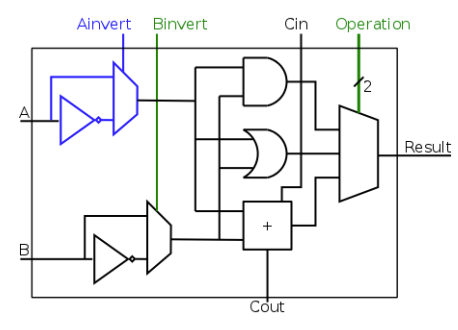
\includegraphics[width=0.7\linewidth]{alu gates.png}
\end{center}
\begin{itemize}
    \item ALUcontrol signal is sent to control ALU
    \item Subtract can be implemented as $A + B' + 1 = A + (-B)$, with the $+ 1$ coming from Cin
    \item NOR is implement as $A' \land B' = (A \lor B)'$ by De Morgan's law
\end{itemize}
\begin{center}
    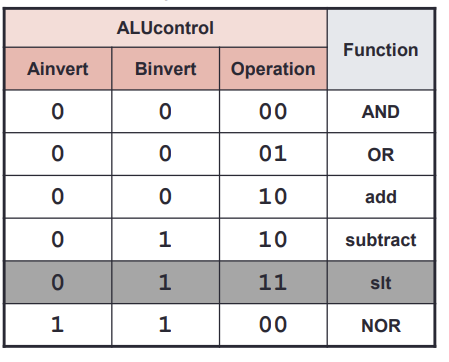
\includegraphics[width=0.7\linewidth]{alu control.png}
\end{center}
\begin{itemize}
    \item Multilevel Decoding
    \begin{itemize}
        \item ALUcontrol depends on 6-bit opcode and 6-bit funct
        \item Brute Force: Use both directly and find expressions with 12 variables
        \item Multilevel Decoding: Use some input to reduce cases, then generate the full output
    \end{itemize}
\end{itemize}

\subsubsection{ALUop}
\begin{itemize}
    \item Use opcode to generate 2-bit ALUop signal
    \item lw / sw : 00 (both use add)
    \item beq: 01 (uses sub)
    \item R-type: 10 (uses funct)
    \item Use ALUop and funct to generate 4-bit ALUcontrol signal
    \item We can ignore some inputs that don't give us any useful information such as F5 and F4
\end{itemize}
\begin{center}
    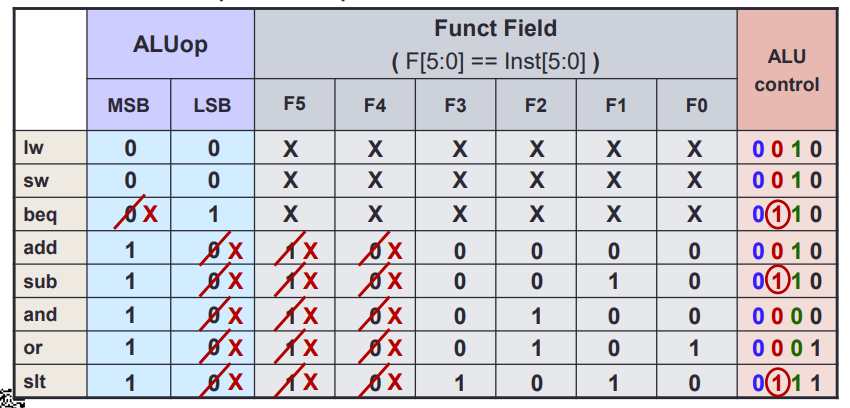
\includegraphics[width=\linewidth]{aluop table.png}
\end{center}

\begin{itemize}
    \item beq is uniquely determined by ALUop 1 = 1
    \item F5 is always 1 for R-format, F4 is always 0
    \item Possible combinational logic:
    \item ALUcontrol 3 = 0
    \item ALUcontrol 2 = $ALUop 0 \lor (ALUop 1 \land F1)$
    \item ALUcontrol 1 = $(\neg ALUop 1) \lor (ALUop 1 \land \neg F2) = \neg ALUop 1 \lor \neg F2$ by De Morgan's law
    \item ALUcontrol 0 = $(F0 \lor F3) \land ALUop 1$
    \item This gives us the following combinational circuit:
\end{itemize}
\begin{center}
    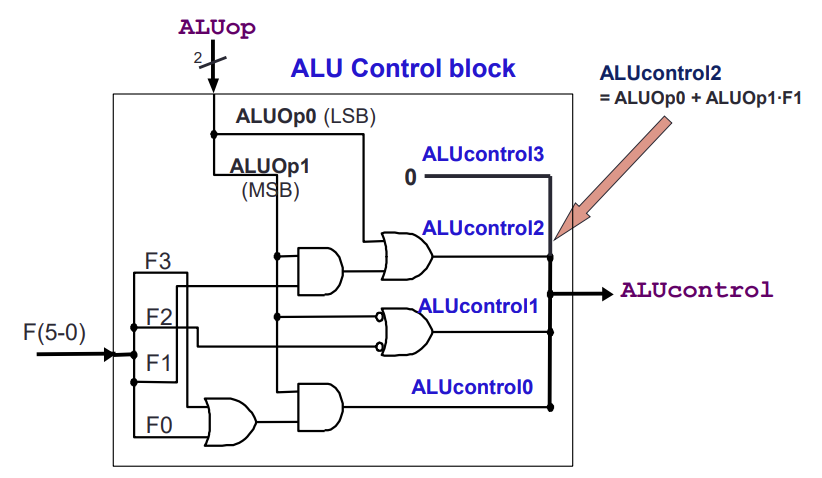
\includegraphics[width=\linewidth]{aluop circuit.png}
\end{center}

\subsubsection{Control Circuit Outputs}
\begin{center}
    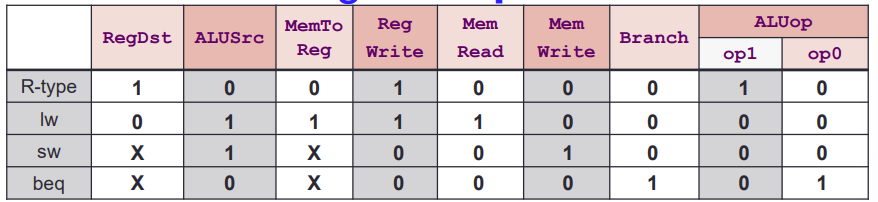
\includegraphics[width=\linewidth]{control outputs.png}
\end{center}

\subsubsection{Control Inputs}
\begin{center}
    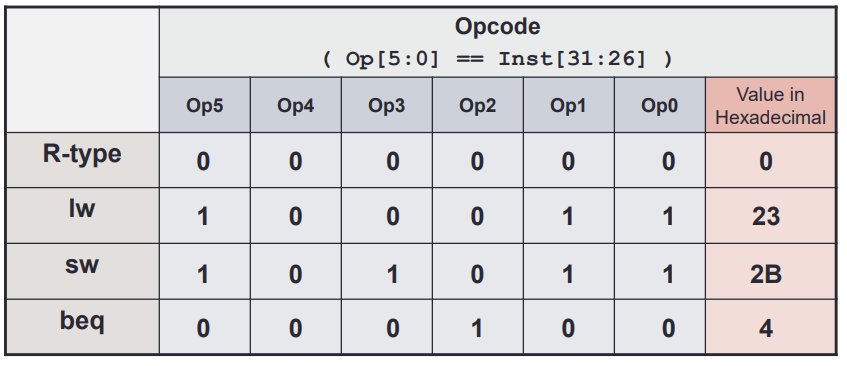
\includegraphics[width=\linewidth]{control inputs.png}
\end{center}

\subsubsection{Control Circuit}
\begin{itemize}
    \item Small circles are inverters
    \item Input are combined using AND gates to determine output of signal based on above tables
\end{itemize}
\begin{center}
    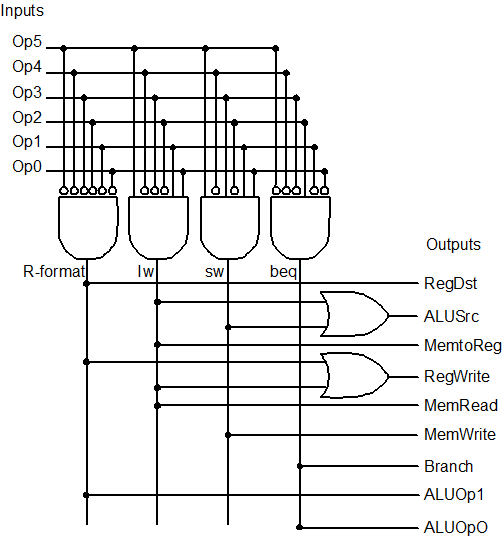
\includegraphics[width=0.7\linewidth]{control circuit.png}
\end{center}

\subsection{Finished Datapath and Control}
\begin{center}
    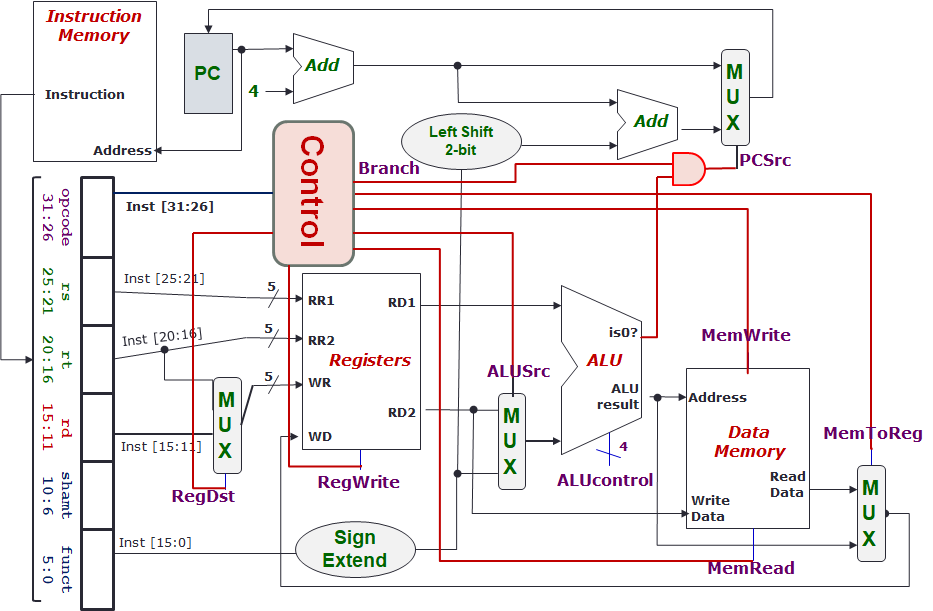
\includegraphics[width=\linewidth]{control}
\end{center}

\begin{itemize}
    \item RR1: rs or Inst[25:21]
    \item RR2: rt or Inst[20:16]
    \item WR: Selected from MUX
    \item WD: Result of final MUX
    \item Opr1: RD1 = R[rs]
    \item Opr2: Selected from either Immd or RD2=R[rt]
    \item Address: ALU result
    \item Write Data: RD2 = R[rt]
\end{itemize}

\subsubsection{Instruction Execution}
\begin{itemize}
    \item Read contents of one or more storage elements
    \item Perform computation through combinational logic
    \item Write results to one or more storage elements
    \item All the steps are performed within a clock period
    \item Writing must be performed during rising edge
    \item Single Cycle Implementation
    \begin{itemize}
        \item All instructions will take as much time as the slowest one
    \end{itemize}
    \item Multicycle Implementation
    \begin{itemize}
        \item Break instructions up into execution steps
        \item Each execution step takes one clock cycle
        \item Cycle time is shorter, clock frequency is higher
        \item Instructions take variable number of clock cycles to complete execution
    \end{itemize}
    \item Pipelining
    \begin{itemize}
        \item Break up the instructions into execution steps, one per clock cycle
        \item Allow different instructions to be in different execution steps simultaneously
    \end{itemize}
\end{itemize}

\section{13. Boolean Algebra}
\begin{itemize}
    \item High/True/1 and Low/False/0
    \item Combinational Circuit: No memory, output depends solely on input
    \item Sequential Circuit: With memory, output depends on both input and current state
    \item AND: $\cdot$, OR: $+$, NOT: $'$
    \item Precedence: NOT > AND > OR
\end{itemize}

\subsection{Laws / Theorems}
\begin{itemize}
    \item Identity Laws: $A+0=0+A=A$, $A\cdot 1 = 1 \cdot A=A$
    \item Inverse/Complement Laws: $A+A'=A'+A=1$, $A\cdot A' = A'\cdot A = 0$
    \item Commutative Laws: $A+B=B+A$, $A\cdot B= B\cdot A$
    \item Associative Laws: $A+(B+C)=(A+B)+C$, $A\cdot(B\cdot C)=(A\cdot B)\cdot C$
    \item Distributive Laws: $A\cdot(B+C)=(A\cdot B)+(A\cdot C)$, $A+(B\cdot C)=(A+B)\cdot(A+C)$
    \item Duality: If AND/OR and 0/1 in an equation are swapped, it remains valid
    \item Idempotency: $X+X=X$, $X\cdot X = X$
    \item One / Zero Element: $X+1=1+X=1$, $X\cdot 0 = 0 \cdot X = 0$
    \item Involution: $(X')'=X$
    \item Absorption 1: $X+X\cdot Y=X$, $X\cdot(X+Y)=X$
    \item Absorption 2: $X+X'\cdot Y=X+Y$, $X\cdot(X'+Y)=X\cdot Y$
    \item DeMorgan's (Can be generalised): $(X+Y)'=X'\cdot Y'$, $(X\cdot Y)'=X'+Y'$
    \item Consensus: $X\cdot Y+X'\cdot Z+Y\cdot Z=X\cdot Y + X' \cdot Z$, $(X+Y)\cdot(X'+Z)\cdot(Y+Z)=(X+Y)\cdot(X'+Z)$
\end{itemize}

\subsection{Standard Forms}
\begin{itemize}
    \item Literal: Boolean variable on its own or in its complemented form
    \item Product Term: A single literal or a logical product of several literals
    \item Sum Term: A single literal or a logical sum of several literals
    \item Sum-of-Products Expression: A product term or a logical sum of several product terms
    \item Product-of-Sums Expression: A sum term or a logical product of several sum terms
    \item Minterm: Product term that contains n literals from all the variables
    \item Maxterm: Sum term that contains n literals from all the variables
    \item Minterm is complement of maxterm
    \item Canonical Form: Unique form of representation
    \item Sum of Minterms: Gather minterms of function where output is 1
    \item Product of Maxterms: Gather maxterms of function where output is 0
    \item Opposite of each other
\end{itemize}

\begin{center}
    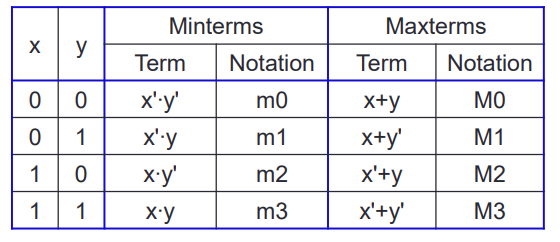
\includegraphics[width=0.7\linewidth]{terms.png}
\end{center}

\section{14. Logic Circuits}
\begin{itemize}
    \item See previous pages for list of logic gates
    \item XOR: Check different, XNOR: Check same
    \item Fan-in: Number of inputs to a gate
    \item Cannot have hanging inputs!
    \item Draw circle for wire intersection
    \item Complete set of logic: Can make any boolean function
    \item e.g. \{AND, OR, NOT\}, \{NAND\}, \{NOR\}
    \item NAND with both inputs $X$ gives $X'$
    \item NAND of NAND(X, Y) gives $X\cdot Y$
    \item NAND (X', Y') gives $X+Y$
    \item Similar for NOR but swap some cases around
    \item SOP: Use 2 level AND-OR or NAND circuit
    \item POS: Use 2 level OR-AND or NOR circuit
\end{itemize}

\section{15. Simplification}
\begin{itemize}
    \item Minimise number of literals
    \item Algebraic Simplification can be hard
\end{itemize}

\subsection{Half Adder}
\begin{itemize}
    \item Adds $(X, Y)$ producing $(C, S)$
    \item $C=X\cdot Y$, $S=X'\cdot Y + X \cdot Y'=X \oplus Y$
\end{itemize}

\begin{center}
    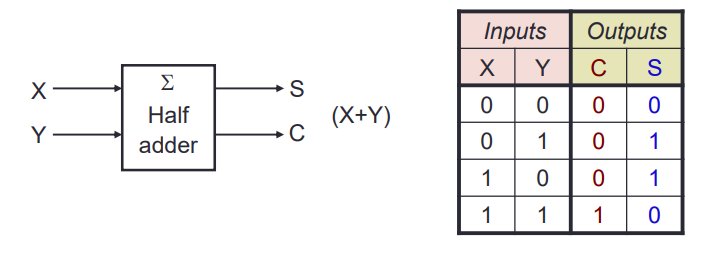
\includegraphics[width=0.7\linewidth]{halfadder.png}
\end{center}

\subsection{K-maps}
\begin{itemize}
    \item Gray Code: Unweighted, only single bit change from one code value to next
    \item K-map: Systematic method to obtain simplified SOP expressions
    \item Each square is a minterm differing by one literal
    \item Has wrap-around
    \item Group as many cells as possible, select as few groups as possible to cover all the cells (minterms) of the function
    \item Implicant: Product term used to cover minterms of function
    \item Prime Implicant: Product term obtaned by combining the maximum possible number of minterms from adjcant squares in the map
    \item Essential Prime Implicants: Prime implicant that includes at least one minterm that is not covered by any other prime implicant
    \item SOP: Select minimum subset of prime implicants to cover minterms, and add them together
    \item Don't Care: Can be either 1 or 0, might help with simplifying k-maps
    \item POS: Draw k-map of complement, then apply DeMorgan's on the result
\end{itemize}

\begin{center}
    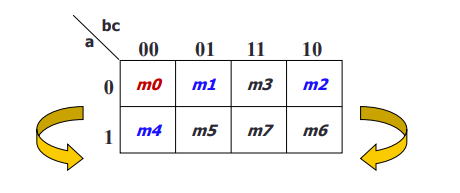
\includegraphics[width=0.7\linewidth]{3varkmap.png}
\end{center}
\begin{center}
    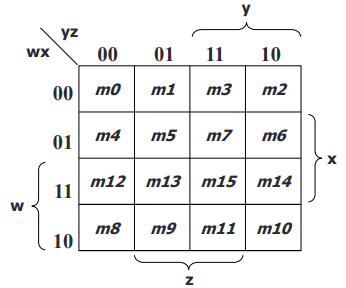
\includegraphics[width=0.7\linewidth]{4varkmap.png}
\end{center}


\section{17. Combinational Circuits}
\subsection{Full Adder}
\begin{itemize}
    \item To fully add two binary numbers, need 3 bits
    \item $C=X\cdot Y+X\cdot Z + Y\cdot Z$, $S=X'\cdot Y' \cdot Z+X'\cdot Y\cdot Z'+X\cdot Y'\cdot Z'+X\cdot Y\cdot Z$
    \item Can be made from 2 half adders and an OR gate
    \item Z is Cin, C is Cout
\end{itemize}

\begin{center}
    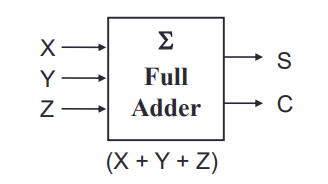
\includegraphics[width=0.7\linewidth]{fulladder.png}
\end{center}
\begin{center}
    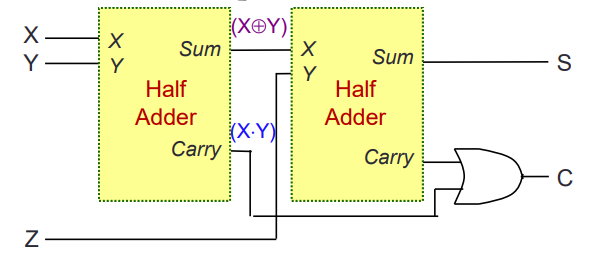
\includegraphics[width=0.7\linewidth]{fulladder2.png}
\end{center}

\subsection{4-bit Parallel Adder}
\begin{itemize}
    \item Add two 4-bit numbers together with Cin to get 5-bit result
    \item Use addition formula for each pair of bits and Cin
    \item $C_{i+1}S_i=X_i+Y_i+C_i$
    \item $C_{i+1}=X_i\cdot Y_i+(X_i\oplus Y_i)\cdot C_i$, $S_i=X_i\oplus Y_i\oplus C_i$
    \item Can use same logic to expand to 16-bit parallel adder
    \item Example Application: Voting system
\end{itemize}

\begin{center}
    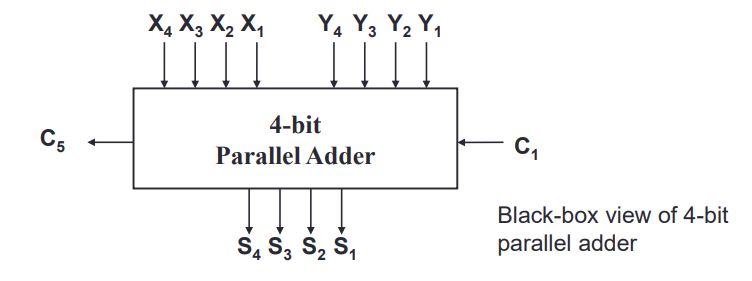
\includegraphics[width=0.7\linewidth]{paralleladder.png}
\end{center}
\begin{center}
    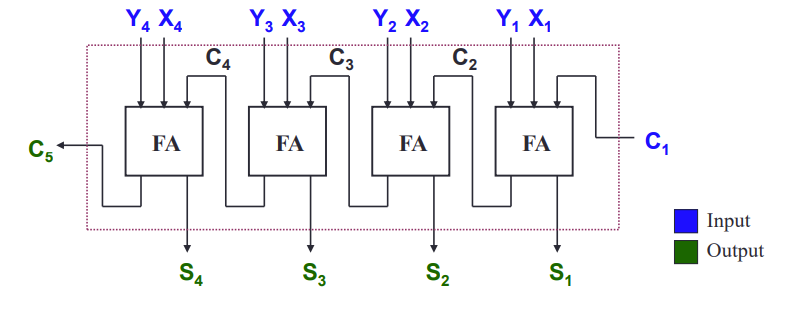
\includegraphics[width=0.7\linewidth]{paralleladder2.png}
\end{center}

\subsection{Magnitude Comparator}
\begin{itemize}
    \item Check trichotomy
\end{itemize}
\begin{center}
    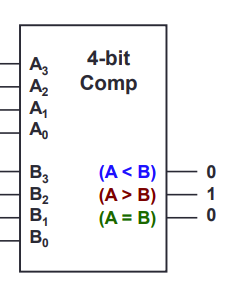
\includegraphics[width=0.7\linewidth]{comparator.png}
\end{center}

\subsection{Circuit Delays}
\begin{itemize}
    \item Max of each input / output
    \item Analyse components
    \item Full adder: If $C_i=mt$, $S_i=max(t, mt)+t$, $C_{i+1}=max(t, mt)+2t$
    \item Parallel Adder: $S_n=(2(n-1)+2)t$, $C_{n+1}=(2(n-1)+3)t$
\end{itemize}

\section{18. MSI Components}
\subsection{Decoder}
\begin{itemize}
    \item Convert binary information from $n$ input lines to $2^n$ output lines, can be used to generate minterms
    \item Implemented with AND gates
    \item We can implement functions by using the output minterms
    \item Can have enable control signal, which is either one/zero-enable
    \item Can build larger decoders from smaller ones
    \item Can also have negated outputs
\end{itemize}

\begin{center}
    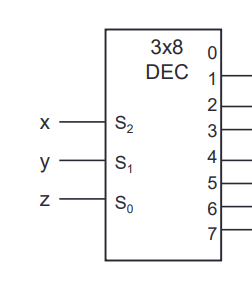
\includegraphics[width=0.7\linewidth]{decoder.png}
\end{center}

\subsection{Encoder}
\begin{itemize}
    \item Opposite of decoding
    \item Provides a code corresponding to input line
    \item Implemented with OR gates
    \item Priority Encoder: Input with highest priority takes precedence, all zero is invalid
\end{itemize}

\subsection{Demultiplexer}
\begin{itemize}
    \item Directs data from input to one selected output line
    \item Identical to decoder with enable using data
\end{itemize}

\begin{center}
    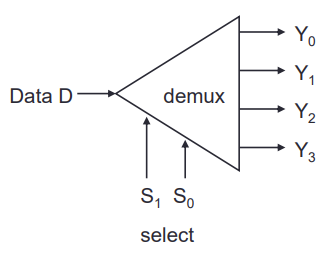
\includegraphics[width=0.5\linewidth]{demultiplexer.png}
\end{center}

\subsection{Multiplexer}
\begin{itemize}
    \item Selects intput from one of the input lines and pipes it to output line
    \item Output is sum of (product of data lines and selection lines)
    \item Larger multiplexers can be constructed from smaller ones
    \item Constructing Function: Connect variables to selection lines, put 1 on data line if it is a minterm, 0 otherwise
    \item Squeezing Multiplexers: Use one variable less by moving it to the input data lines
    \item Group inputs by selector lines, and determine MUX input based on remaining variable and function
\end{itemize}

\begin{center}
    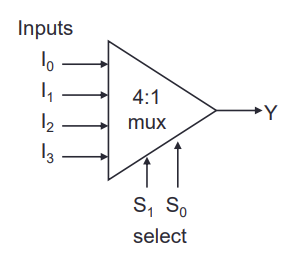
\includegraphics[width=0.5\linewidth]{multiplexer.png}
\end{center}
\begin{center}
    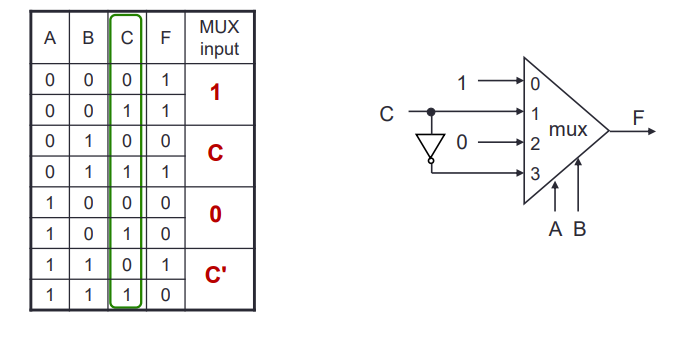
\includegraphics[width=0.7\linewidth]{squeeze.png}
\end{center}

\section{19. Sequential Logic}
\begin{itemize}
    \item Syncronous: Outputs change at specific time, Asynchronous: Outputs change at any time
    \item Multivibrator: Class of sequential circuits, Bistable, Monostable, Astable
    \item Bistable logic devices: Latches and flip flops
    \item Memory Element: Device which can remember value indefinitely, or change value on command from inputs
    \item Clock: Usually a Square Wave
    \item Memory Element can be Pulse Triggered (Latches) or Edge triggered (Flip-flops)
    \item Flip-flops are synchronous bistable devices, and have a $>$ indicating clock input
\end{itemize}

\subsection{S-R Latch}
\begin{itemize}
    \item Inputs: $S, R$, Outputs: $Q, Q'$
    \item $Q$ high: SET state, $Q$ low: RESET state
    \item Gated: Has enable input, outputs can only change if enabled
\end{itemize}
\begin{center}
    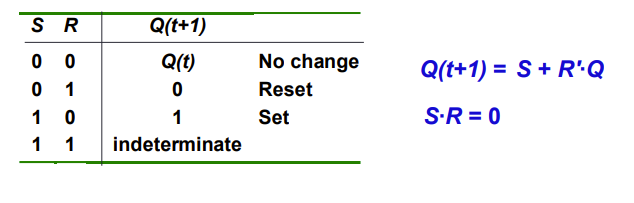
\includegraphics[width=0.7\linewidth]{srlatch.png}
\end{center}

\subsection{Gated D Latch}
\begin{itemize}
    \item S-R latch, but $R=S'$
    \item Eliminates invalid state
\end{itemize}
\begin{center}
    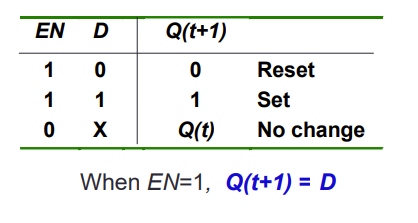
\includegraphics[width=0.7\linewidth]{dlatch.png}
\end{center}

\subsection{Asynchronous Inputs}
\begin{itemize}
    \item Affect state of flip-flop independent of clock
    \item Preset immediately sets output to HIGH
    \item Clear immediately sets output to LOW
\end{itemize}

\subsection{Flip-Flops}
\subsubsection{Characteristic Table}
\begin{center}
    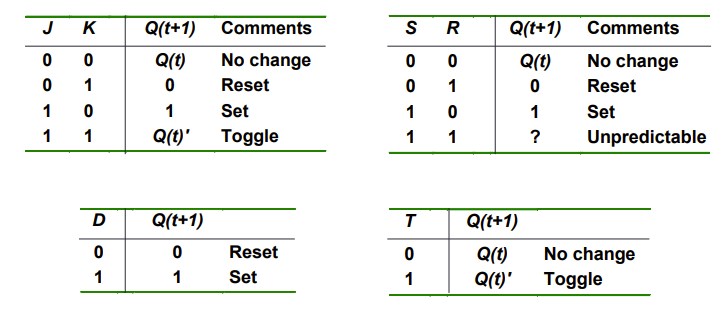
\includegraphics[width=\linewidth]{flipflopc.png}
\end{center}
\subsubsection{Excitation Table}
\begin{center}
    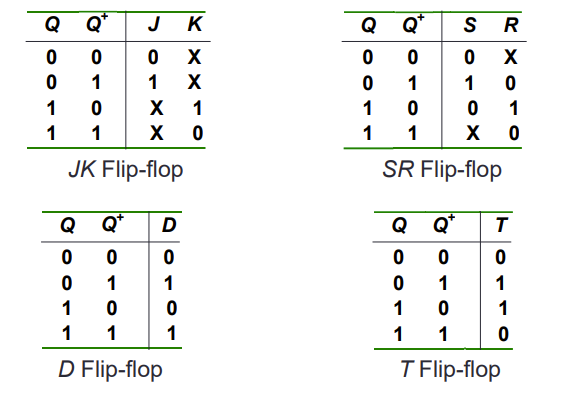
\includegraphics[width=\linewidth]{flipflope.png}
\end{center}
\subsubsection{State Table and State Diagram}
\begin{itemize}
    \item Use K-map to find flip-flop input functions based on current state and input
    \item Edge is input/output
    \item Nodes are states
\end{itemize}
\begin{center}
    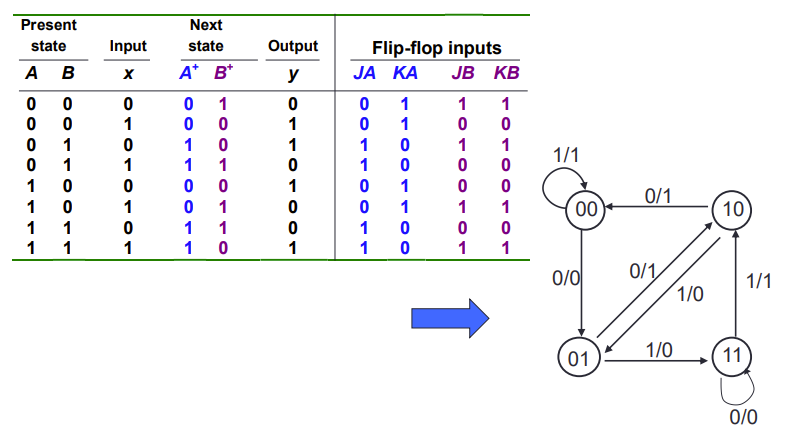
\includegraphics[width=\linewidth]{statediagram.png}
\end{center}

\subsection{Memory}
\begin{itemize}
    \item stores program and data
    \item 1 byte = 8 bits, 1 word is a multiple of bytes
    \item Hierarchy: Fast expensive volatile to Slow cheap non-volatile
    \item Memory unit stores information in words
    \item Has input (write) lines and output (read) lines
    \item Address consists of lines to choose location
    \item Static RAM: Uses flip-flops as memory cells, Dynamic RAM: Uses capacitor charges to represent data, have to be constantly refreshed
    \item Memory Array: Chips combined to form larger memory
\end{itemize}

\section{20. Pipelining}
\begin{itemize}
    \item Does not help latency of single tasks, but rather throughput of entire workload
    \item Multipled tasks operating simultaneously using different resources
    \item Delays are due to slowest stage and stalling for dependencies
    \item Introduce Pipeline registers between stages
\end{itemize}
\begin{center}
    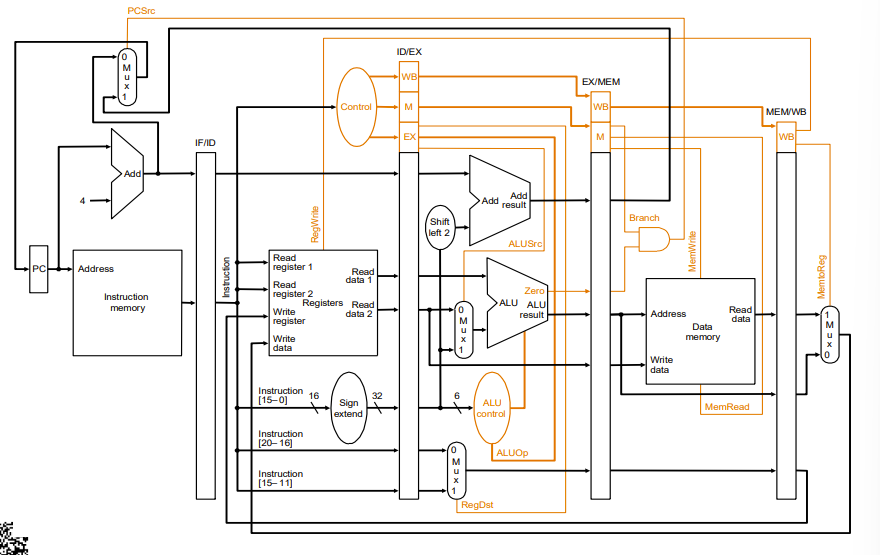
\includegraphics[width=\linewidth]{pipeline.png}
\end{center}
\begin{itemize}
    \item Stages and information:
    \begin{itemize}
        \item ID Stage: IF/ID supplies register numbers, offset, PC+4, ID/EX receives data values from register file, extended immediate, PC+4
        \item EX Stage: ID/EX supplies above, EX/MEM receives (PC+4)+(Immd x 4), ALU result, isZero?, Data Read 2
        \item MEM Stage: EX/MEM supplies above, MEM/WB receives ALU result, memory read data
        \item WB Stage: MEM/WB supplies above, at the end, result is written back to register file
        \item However, register provided by IF/ID is wrong, so we need to pass it from ID/EX all the way through
    \end{itemize}
    \item Each control signal has an associated stage
    \item Single-Cycle Processor: Cycle Time = max(Total of time for each stage) for each instruction, Execution time for I instructions is multiplied
    \item Multi-Cycle Processor: Cycle Time = max(Time for a stage), Execution time for I instructions = I x Average Cycles per Instruction x Cycle Times
    \item Pipelining Processor: Cycle Time = max(Time for a stage) + Pipelining Overhead, Cycles for I instructions = I + N - 1, Execution time for I instructions = (I + N - 1) x Cycle Time
    \item Ideal Speedup: Each stage takes same amount of time, no pipelining overhead, number of instructions is much larger than number of stages, gives N times speedup
\end{itemize}

\subsection{21. Pipeline Hazards}
\subsubsection{Structural Hazard}
\begin{itemize}
    \item Simultaneous use of hardware resource
    \item e.g. If only single memory, memory could be accessed at the same time by 2 different instructions
    \item Stalling: Delay instruction for a cycle
    \item Separate Memory: Split memory into data and instruction memory
    \item Writing and Reading from memory at same time: Split cycle into half, first half for writing and second half for reading
\end{itemize}

\subsection{Instruction Dependencies}
\subsubsection{Data Dependencies}
\begin{itemize}
    \item Overlap between data accessed by different instructions
    \item Read After Write / True data dependency: Later instruction reads from destination register written by earlier instruction
    \item Write after read, Write after write, do not cause pipeline hazards
    \item Result from execution is produced at end of EX stage, and only needed at start of EX stage of next instruction
    \item Solution: Forward the result to any later instructions, bypassing data read or ID
    \item However, this does not work for the result of LOAD instructions after MEM stage, so we still need stalling
\end{itemize}

\subsubsection{Control Dependencies}
\begin{itemize}
    \item Execution of instruction depends on another
     \item Control Dependency: Branch decision is made in MEM stage
    \item Stalling: Waiting until after MEM stage to fetch next instruction, introduces 3 cycle delay
    \item Techniques: Early branch resolution, Branch prediction, Delayed branching
    \item Early Branching: Make decision in ID stage instead of MEM, reduced to 1 cycle delay
    \item However, registers involved might be produced by instructions before, and further stalling might be needed
    \item Solve by adding forwarding path from ALU to ID stage, still has 1 cycle delay
    \item After a load instruction, early branching does not speedup
    \item Branch Prediction: Assume all branches are not taken
    \item If wrong guess is made, flush instructions
    \item Delayed Branching: Move non-control dependent instructions into slots following a branch (branch-delay slots)
    \item Executed regardless of outcome, if no such instruction, add no-op
    \item With early branching, we have 1 slot
\end{itemize}

\subsection{Summary}
\begin{itemize}
    \item Default: Wait till after MEM then get result in ID
    \item Forwarding: Forward from EX to next EX, or MEM to next EX
    \item Default: Wait till after MEM to get result to IF next instruction
    \item Early Branching: Compute result in ID, forward from previous EX
    \item Branch Prediction: Carry on and fetch next instruction, fetch correct instruction immediately after actual result is known
    \item List of delay durations:
\end{itemize}
\begin{center}
    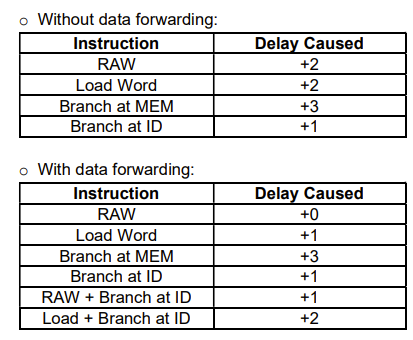
\includegraphics[width=0.8\linewidth]{delays.png}
\end{center}

\section{22. Cache}
\begin{itemize}
    \item Keep frequently and recently used data in smaller but faster memory
    \item Principle of Locality: Program access only a small portion of the memory address space within a small time interval
    \item Temporal Locality: Recently referenced items are likely to be referenced again soon
    \item Spatial Locality: Nearby items are likely to be referenced soon
    \item Cache Hit: Data is in cache, Rate: Fraction of memory access that hit, Time: Time to access cache
    \item Cache Miss: Data is not in cache, Rate: 1 - Hit rate, Penalty: Time to replace cache block + hit time
    \item Average Access Time = Hit Rate * Hit Time + (1 - Hit Rate) * Miss Penalty
    \item Cache Block/Line: Unit of transfer between memory and cache, typically one or more words
    \item MIPS: 1 word = 4 bytes = 32 bits
    \item Memory Address = (32-N) Block Number + N Offset
\end{itemize}

\subsection{Direct Mapped Cache}
\begin{itemize}
    \item Cache Index = Block Number mod Number of Cache Blocks
    \item If Number of Cache Blocks = $2^M$, then the last M bits are the cache index
    \item Multiple memory blocks can map to the same cache block when they have the same cache index
    \item They have different Tag = Block Number / Number of Cache Blocks
    \item If Cache Block Size = $2^N$ bytes and Number of Cache Blocks = $2^M$, then Memory Address = (32-N-M) bits Tag, M bits Index, N bits offset
    \item Block Number = Tag + Index bits
    \item Cache also has a valid bit indicating validity of data
    \item Example:
    \begin{itemize}
        \item e.g. 4GB Memory, 16KB Cache, 16 byte blocks
        \item Offset = $N = 2^4$ bits, Block Number = 32 - 4 = 28 bits
        \item Number of Blocks = $2^{28}$
        \item Number of Cache Blocks = 1024 = $2^{10}$
        \item Cache Index = $M = 10$ bits
        \item Cache Tag = 32 - 10 - 4 = 18 bits
    \end{itemize}
    \item Offset = log2 Number of bytes in Block
    \item Number of Cache Blocks = Cache Size / Block Size
    \item Cache Index = log2 Number of Cache Blocks
    \item Tag = 32 - Offset - Cache Index
    \item Compulsory / Cold Miss: First access to block, needs to be brought into cache
    \item Conflict / Collision Miss: Several blocks are mapped to same block or set
    \item Capacity Miss: Blocks are discarded as cache cannot contain all blocks needed
    \item Cache and main memory could be inconsistent
    \item Write-through: Write data both to cache and to main memory
    \item Limited by memory speed, can use write buffer to speedup
    \item Write-back: Write data to cache, and only to main memory when evicted
    \item Wasteful if we write back every block, can use dirty bit to indicate whether data is changed
    \item On read miss, data loaded into cache and then loaded into register
    \item Write Allocate: Load complete block into cache, change only required word in cache, write to main memory depending on policy
    \item Write Around: Do not load block to cache, write directly to main memory only
\end{itemize}
\begin{center}
    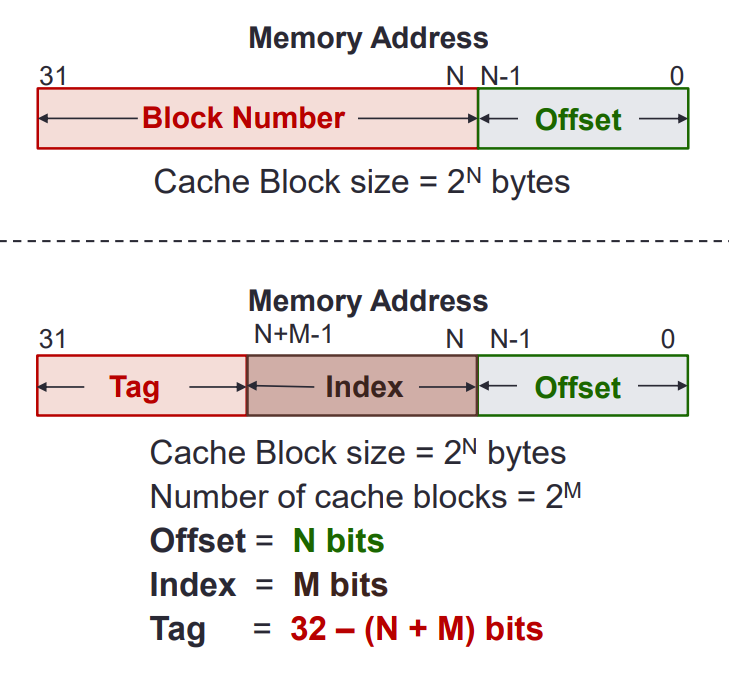
\includegraphics[width=0.8\linewidth]{directcache.png}
\end{center}

\section{23. Set / Fully Associative Cache}
\subsection{Set Associative Cache}
\begin{itemize}
    \item Block Size tradeoff: Large block size takes advantage of spatial locality, but larger miss penalty, and fewer blocks increases miss rate
    \item Set Associative Cache targets conflict misses
    \item N-way Set Associative Cache: Memory block can be in a fixed number of locations in cache
    \item Cache contains a number of sets, each with N blocks
    \item Memory block can be place in any of the N blocks after loading
    \item Cache Set Index = Block Number mod Number of Cache Sets
    \item Essentially the same as direct mapping bit and math wise
    \item Number of Sets = Cache Blocks / N-way
    \item Set Index = log2 Number of Sets
    \item Rule of Thumb: A direct mapped cache of size N has about the same miss rate as a 2-way set associative cache of size N/2
\end{itemize}
\begin{center}
    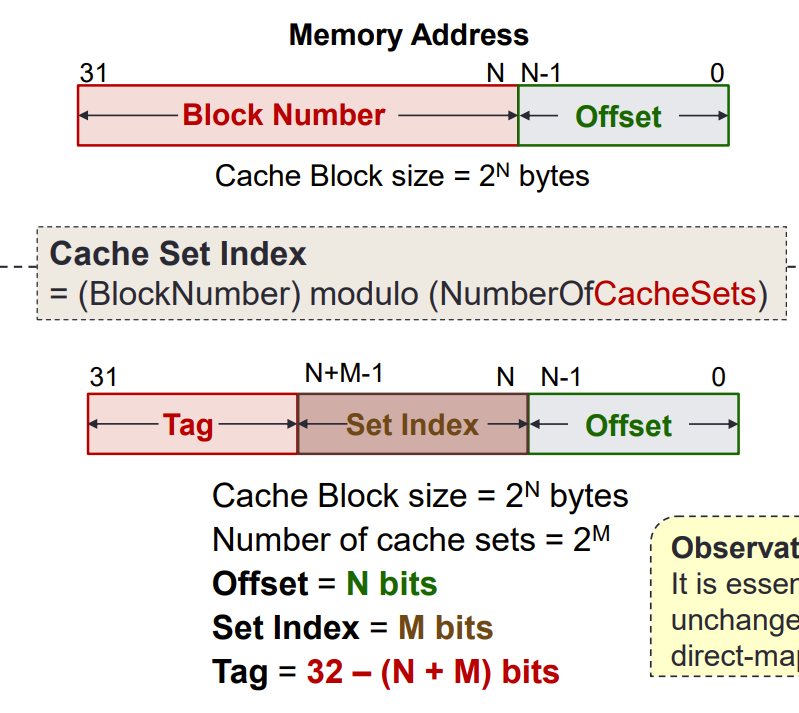
\includegraphics[width=0.8\linewidth]{setcache.png}
\end{center}

\subsection{Fully Associative Cache}
\begin{itemize}
    \item Memory block can be placed in any location in cache
    \item Cache Block size = $2^N$ bytes
    \item Number of Cache blocks = $2^M$
    \item Offset = N bits, Tag = 32 - N bits
\end{itemize}
\begin{center}
    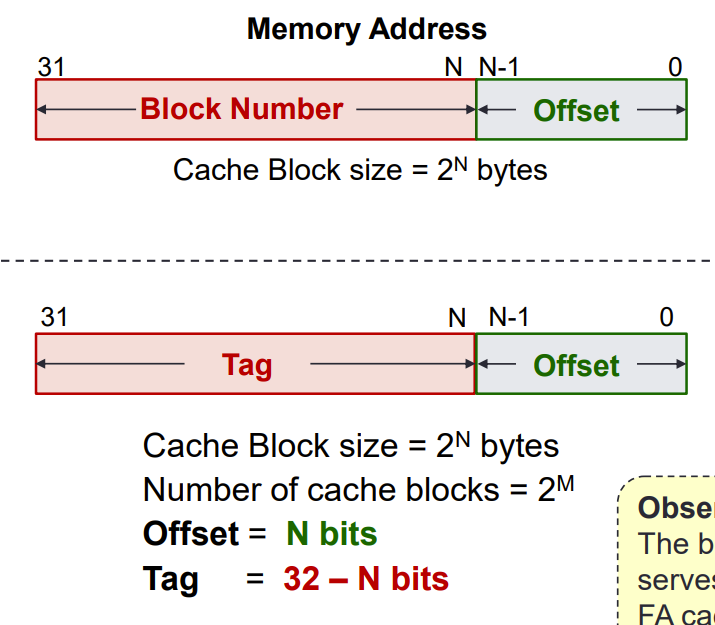
\includegraphics[width=0.8\linewidth]{fullcache.png}
\end{center}

\subsection{Performance / Replacement Policy}
\begin{itemize}
    \item Total Miss = Cold Miss + Conflict Miss + Capacity Miss
    \item Capacity Miss = Total Miss - Cold Miss when Conflict Miss = 0
    \item Conflict miss is 0 for fully associative cache
    \item Set Associative / Fully Associative Cache needs to replace blocks if full using block replacement policy
    \item Least Recently Used: Temporal Locality
    \item First in First Out, Random Replacement, Least Frequently Used
\end{itemize}
\begin{center}
    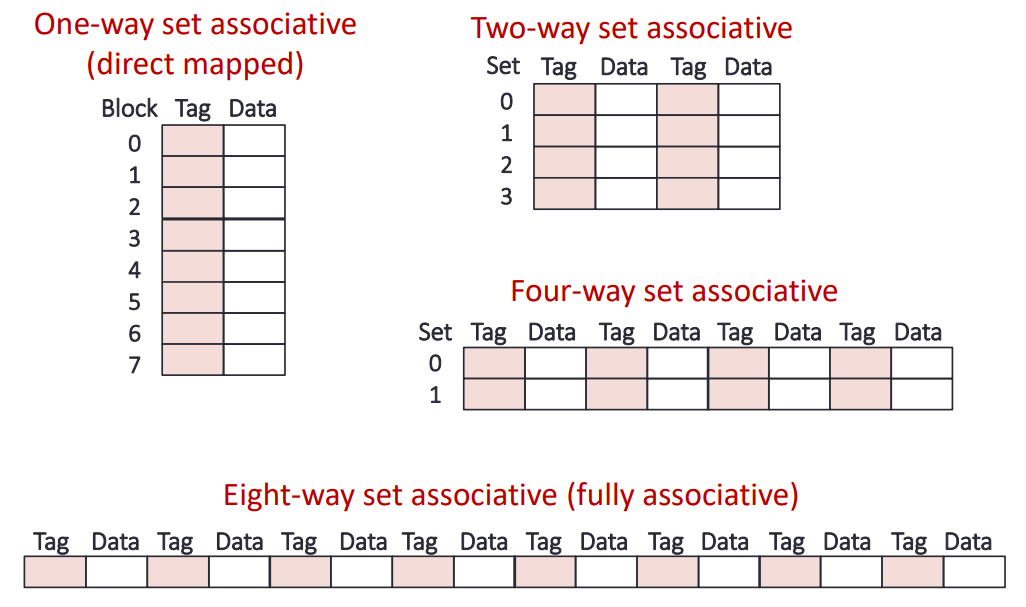
\includegraphics[width=0.8\linewidth]{cache.png}
\end{center}
\end{multicols*}
\end{document}